
$\because \triangle ABC$ is isosceles, its vertices are
\begin{align}
\vec{C} = \myvec{0\\0},
\vec{A} = \myvec{6\\0}, 
\vec{B} = \myvec{0\\6}
\end{align}
which are used to plot the desired triangle in Fig. \ref{constr/26/fig:right_angle_triangle}.	
%
\begin{figure}[!ht]
\centering
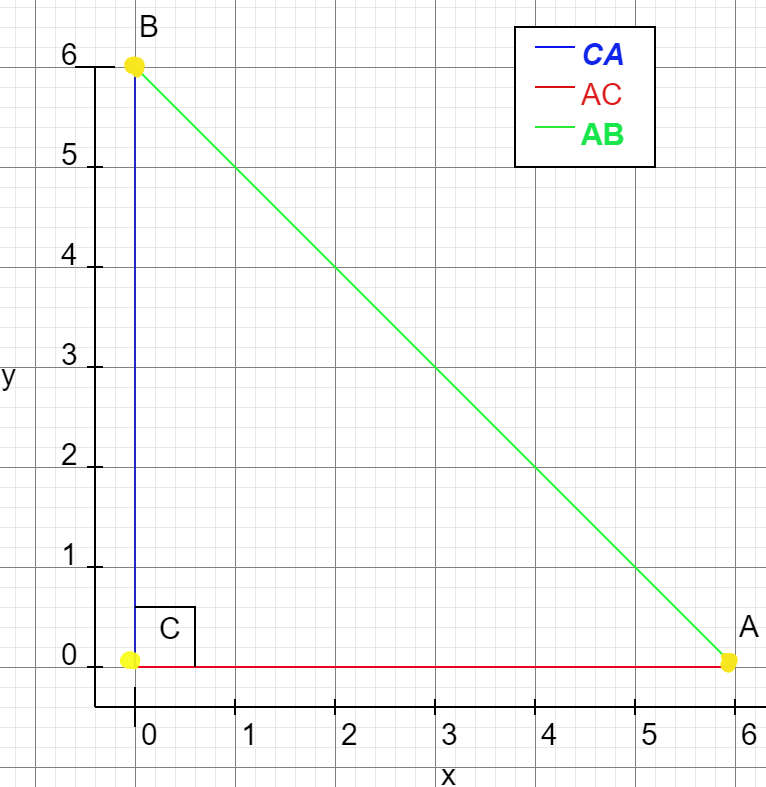
\includegraphics[width=\columnwidth]{solutions/26/diagram-1.png}
\caption{Isosceles Right Angle $\triangle ABC$}
\label{constr/26/fig:right_angle_triangle}	
\end{figure}

